\section[相似变换]{相似变换\\Similarity Transformations}	
\par\noindent
In the previous section we suspended the rank defect of $A^\mathsf{T}A$ by a bordering matrix $G$.At the same time we added constraints on the least-squares problem. These constraints
were also described by $G$! However, the constraints may be of a more general form. In this
section we shall introduce constraints which transform the free network to one with at least
$d$ postulated coordinates and we shall derive the pertinent formulas. The related covariance
matrix $\sum_{transformed}$ is correspondingly transformed, and consequently $d$ columns and rows will be zeroed. We start by working through a simple example.
\begin{figure}
	\centering
	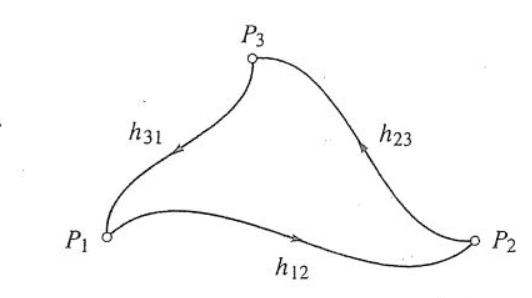
\includegraphics[width=0.7\linewidth]{TeX_files/Part02/chapter07/image/7-4}
	\caption{Figure 7.4 Simple free leveling network}
	\label{fig:7-4}
\end{figure}

\textbf{Example 7.6} $A$ simple leveling network has three nodes $P_1$ , $P_2$, and $P_3$ and observed oriented differences of heights $h_{12}$, $h_{23}$, and $h_{31}$, see Figure 7.4. According to the loop law we have
\begin{equation}
h_{12} + h_{23} + h_{31} = 0.
\end{equation}
We cannot calculate the heights of the nodes from these differences. So we choose $P_1$ as
reference point,i.e. we put $P_1$ = given constant = $h_1$. The best estimate for $h_2$ and $h_3$ is now unique
\begin{equation}
h_{i} = h_{1i} + h_{1} = h_{i}^{1} + h_1,\qquad i = 1,2,3
\end{equation}
where the upper index refers to the reference point chosen. Yet there is a slight flaw because
of the arbitrariness of $P_1$ as reference. In fact we can take any point of the network as
reference point. We can even choose the barycenter $P_b$ and assign it the height
\begin{equation*}
h_{b} = \frac{1}{n}\sum_{i = 1}^{n}h_i.
\end{equation*}
That choice leads to
\begin{equation*}
h_{i} = \frac{1}{3}(h_{1i} + h_{2i} + h_{3i}) + h_b = h_{i}^{b} + h_b.
\end{equation*}
All sets of heights like $h_{i}^{1}$ or $h_{i}^{b}$ can be looked upon as valid heights. So it is more a question what set to choose.However,the statistical properties of the heights $h_{i}^{1}$ or $h_{i}^{b}$ depend highly on the choice of reference point. From $E{h_{3}^{1}} = E{h_{3}^{1} + h_{2}^{3}}$ and $E{h_{3}^{b}} = E{\frac{2}{3}h_{1}^{2} + h_{2}^{3} + \frac{1}{3}h_{1}^{3}}$ follows for instance that $E{h_{3}^{1}} \neq E{h_{3}^{b}}$.Their covariances differ,too.
\par
When comparing two sets of heights it is essential that they refer to the same level of
reference. So in order to do this we shall learn how to transform heights from one system
to another. We write (7.28) explicitly
\begin{equation}
\begin{bmatrix}
h_{1}\\
h_{2}\\
h_{3}
\end{bmatrix}
= \begin{bmatrix}
h_{1}^{1}\\
h_{2}^{1}\\
h_{3}^{1}
\end{bmatrix}
+ \begin{bmatrix}
1 & 0 & 0\\
1 & 0 & 0\\
1 & 0 & 0
\end{bmatrix}
\begin{bmatrix}
h_{1}\\
h_{1}\\
h_{1}
\end{bmatrix}
\end{equation}
or
\begin{equation}
\begin{bmatrix}
h_{1}^{1}\\
h_{2}^{1}\\
h_{3}^{1}
\end{bmatrix}
=\begin{bmatrix}
\quad0 & \quad0 & \quad0\\
-1 & \quad1 & \quad0\\
-1 & \quad0 & \quad1
\end{bmatrix}
\begin{bmatrix}
h_{1}\\
h_{2}\\
h_{3}
\end{bmatrix}
\end{equation}
Equation (7.30) shows us how we can transform from one height system, say $h_{i}^{1}$, to the
height system defined by $P_1$ as reference point. In a similar way we obtain
\begin{equation*}
\begin{bmatrix}
h_{1}^{b}\\
h_{2}^{b}\\
h_{3}^{b}
\end{bmatrix}
=\frac{1}{3}
\begin{bmatrix}
\quad2 & -1 & -1\\
-1 & 2 & -1\\
-1 & -1 & \quad2
\end{bmatrix}
\begin{bmatrix}
h_{1}^{1}\\
h_{2}^{1}\\
h_{3}^{1}
\end{bmatrix}
\end{equation*}
and in general
\begin{equation}
\begin{bmatrix}
h_{1}^{b}\\
h_{2}^{b}\\
\vdots\\
h_{n}^{b}
\end{bmatrix}
=\frac{1}{n}
\begin{bmatrix}
n - 1 & -1 & \ldots&-1\\
-1 &  n - 1& \ldots&-1\\
\vdots&\vdots&\ddots&\vdots\\
-1 & -1 &\ldots&   n - 1
\end{bmatrix}
\begin{bmatrix}
h_{1}^{1}\\
h_{2}^{1}\\
\vdots\\
h_{n}^{1}
\end{bmatrix}
\end{equation}
This square matrix is already seen for $n = 5$ in Example 7.3.
\par
The 2-dimensional transformation model must allow for two translations $t_x, t_y$, a
rotation $r_\varphi$, and a change of scale $s_k$. The \emph{similarity transformation} from $(x , y)$ to $(\xi, \eta)$(the ��from�� and ��to�� systems in geodesy) is given by
\begin{equation}
\begin{bmatrix}
\xi_{i}\\
\eta_{i}
\end{bmatrix}
=
\begin{bmatrix}
\ a & b\\
-b & a
\end{bmatrix}
\begin{bmatrix}
x_i\\
y_i
\end{bmatrix}
+   \begin{bmatrix}
t_x\\
t_y
\end{bmatrix}
\end{equation}
The $2p$ observation equations resulting from $p$ common points are
\begin{equation}
\begin{bmatrix}
x_1 & y_1 & 1 & 0\\
x_2 & y_2 & 1 & 0\\
&\vdots\\
x_p & y_p & 1 & 0\\
y_1 &-x_1 & 0 & 1\\
y_2 &-x_2 & 0 & 1\\
&\vdots\\
y_p &-x_p & 0 & 1
\end{bmatrix}
\begin{bmatrix}
a\\
b\\
t_x\\
t_y
\end{bmatrix}
=
\begin{bmatrix}
\xi_1\\
\xi_2\\
\vdots\\
\xi_p\\
\eta_1\\
\eta_2\\
\vdots\\
\eta_p
\end{bmatrix}
-
\begin{bmatrix}
e\xi_1\\
e\xi_2\\
\vdots\\
e\xi_p\\
e \eta_1\\
e\eta_2\\
\vdots\\
e\eta_p
\end{bmatrix}
\end{equation}
or symbolically
\begin{equation*}
Af = b - e.
\end{equation*}
This linear least-squares problem does not show any difficulties.
\par
Yet, we cannot resist demonstrating the classical solution procedure. We set all
weights to unity and the normal equations $A^\mathsf{T}Af = A^\mathsf{T}b$ can be written
\begin{equation}
\begin{bmatrix}
\sum(x_{i}^{2} + y_{i}^{2}) & 0 & \sum x_i & \sum y_i\\
0 & \sum(x_{i}^{2} + y_{i}^{2}) & \sum y_i & -\sum x_i\\
\sum x_i & \sum y_i & p & 0\\
\sum y_i &-\sum x_i & 0 & p
\end{bmatrix}
\begin{bmatrix}
a\\
b\\
t_x\\
t_y
\end{bmatrix}
=
\begin{bmatrix}
\sum(\xi_ix_i + \eta_iy_i)\\
\sum(\xi_iy_i - \eta_ix_i\\
\sum\xi_i\\
\eta_i
\end{bmatrix}.
\end{equation}
All summations run from 1 to $p$. For numerical reasons we reduce the coordinates in both
systems to their respective barycenters $(x_s, y_s)$ and $(\xi_s, \eta_s)$. This leads to $\sum_{x_i} = \sum_{y_i} = \sum_{\xi_i} = \sum_{\eta_i} \equiv 0$ and $A^\mathsf{T}A$ becomes diagonal. We introduce starred coordinates relative to the barycenter$x_{i}^{*} = x_i - x_s, y_{i}^{*} = y_i - y_s$, with $x_s = \sum x_i/p, y_s = \sum y_i/p$:
\par
Now the inversion reduces to solving individual equations:
\begin{equation*}
\begin{bmatrix}
\star & 0 & 0 & 0\\
0 & \star & 0 & 0\\
0 & 0 & p & 0\\
0 & 0 &0 & p
\end{bmatrix}
\begin{bmatrix}
a\\
b\\
t_x\\
t_y
\end{bmatrix}
=
\begin{bmatrix}
\star\\
\star\\
0\\
0
\end{bmatrix}.
\end{equation*}
Nonzero entries are marked by $\star$. The explicit solution can be written
\begin{equation}
\hat{a} = \frac{\sum(\xi_{i}^{\ast} x_{i}^{\ast} + \eta_{i}^{\ast} y_{i}^{\ast})}
{\sum{(x_{i}^{\ast}}^{2}  + {y_{i}^{\ast}}^{2})}
\qquad \text{and} \qquad
\hat{b} = \frac{\sum(\xi_{i}^{\ast} y_{i}^{\ast} - \eta_{i}^{\ast} x_{i}^{\ast})}
{\sum{(x_{i}^{\ast}}^{2}  + {y_{i}^{\ast}}^{2})}
\end{equation}
Next, we can determine
\begin{equation}
\hat{k} = \sqrt{{\hat{a}}^2 + {\hat{b}}^2}
\qquad \text{and} \qquad
\hat{\varphi} = \arctan{\hat{b} / \hat{a}}.
\end{equation}
Finally we get $\hat{t}_x$ and $\hat{t}_y$ from (7.34):
\begin{equation}
\hat{t}_x = \frac{\sum \xi_i - \hat{a}\sum x_i - \hat{b}\sum y_i}{p}
= \xi_s - \hat{a}x_s - \hat{b}y_s,
\end{equation}
\begin{equation}
\hat{t}_y = \frac{\sum \eta_i - \hat{a}\sum y_i + \hat{b}\sum x_i}{p}
= \eta_s - \hat{a}y_s + \hat{b}x_s.
\end{equation}
The covariance matrix for $\hat{f}$ involves $A = p\sum(x_{i}^{2} + y_{i}^{2})
- (\sum x_{i})^{2}- (\sum y_{i})^{2}$ :
\begin{equation*}
\sum\nolimits_{\hat{f}} = \frac{1}{A}
\begin{bmatrix}
\ p       & \ 0        & -\sum x_i                      &-\sum y_i\\
\ 0       & \ p        & \ -\sum y_i                    &\ \sum x_i\\
-\sum x_i & -\sum y_i  & \ \sum(x_{i}^{2} + y_{i}^{2})  &\ 0\\
-\sum y_i & \ \sum x_i & \ 0                            &\ \sum(x_{i}^{2} + y_{i}^{2})
\end{bmatrix}.
\end{equation*}
The variance of unit weight is also the variance in transformed coordinates. According to
(4.79) this is
\begin{equation*}
\hat{\sigma}_{0}^{2} = \frac{\sum(e_{\xi_i}^{2} + e_{\eta_i}^{2})}{2p - 4}.
\end{equation*}
For the translations we have
\begin{equation}
\hat{\sigma}_{\hat{t}_x} = \hat{\sigma}_{\hat{t}_y}
= \hat{\sigma}_0\sqrt{\frac{\sum(x_{i}^{2} + y_{i}^{2})}{p\sum(x_{i}^{2} + y_{i}^{2})
		- (\sum x_{i})^{2} - (\sum y_{i})^{2}}}
= \hat{\sigma}_0\sqrt{\frac{1}{p} + \frac{x_{s}^{2} + y_{s}^{2}}{{\sum({x_{i}^\ast}}^{2} + {y_{i}^{\ast}}^{2})}}.
\end{equation}
Observe that the standard deviations for $\hat{t}_x$ and $\hat{t}_y$ not only depend on $p$, as expected, but also on the position of the origin.
\par
Thus we have described the most important, elementary circumstances about the similarity transformation. It includes $p$ points whose coordinates are given in two systems,namely an original $x$,$y$ system and a different $\xi$,$\eta$ system. The transformation parameters
$\hat{k}, \hat{\varphi}, \hat{t}_x$ and $\hat{t}_y$ are estimated through a least-squares procedure. Additionally, the solution makes it possible to transform any other point$(x_j,y_j)$ into the corresponding $(\xi_i,\eta_j)$ by means of the transformation equations
\begin{equation}
\xi_j
= \hat{a}x_j + \hat{b}y_{j} + \hat{t}_x,\qquad
\eta_j = -\hat{b}x_j + \hat{a}y_{j} + \hat{t}_y.
\end{equation}
\textbf{Example 7.7} We shall demonstrate the procedure just described by a numerical example.
Suppose we know the exact coordinates $(N, E) = (\xi, \eta)$ and $(X, Y)$ of 7 common points.
We want to determine the transformation parameters and to transform a single point with
given $x, y$ coordinates. The procedure is in fact a 2-dimensional interpolation.
\par
\begin{table}[htbp]
	% \caption{\label{tab:test}}
	\begin{tabular}{ccccc}
		\toprule
		\multirow{2}{*}{Point} & $x_i$ & $y_i$ & $\xi_{i}$ & $\eta_i$ \\
		{} &[m] & [m] & [m] & [m]\\
		\midrule
		62-04-005 &277 722.022  &-230 855.152 & 6 310 000.527 &562 940.820\\
		62-04-801 &275 956.869  &-231 105.839 & 6 308 231.260 &562 725.625\\
		62-04-810 &277 563.374  &-235 447.400 & 6 309 749.964 &558 354.121\\
		62-04-811 &278 608.525  &-233 945.915 & 6 310 824.656 &559 833.890\\
		62-04-815 &276 163.682  &-236 471.626 & 6 308 330.475 &557 358.463\\
		63-01-002 &273 578,801  &-230 941.425 & 6 305 857.705 &562 937.589\\
		63-04-003 &274 533.958  &-235 063.723 & 6 306 729.799 &558 798.283\\
		$s$       &276 303.890  &-233 404.440 & 6 308 532.055 &560 421.256\\
		\bottomrule
	\end{tabular}
\end{table}
\begin{table}[htbp]
	% \caption{\label{tab:test}}
	\begin{tabular}{ccccc}
		\toprule
		\multirow{2}{*}{Point} & $x_{i}^{\ast}$ & $y_{i}^{\ast}$ & $\xi_{i}^{\ast}$ & $\eta_{i}^{\ast}$ \\
		{} &[m] & [m] & [m] & [m]\\
		\midrule
		62-04-005 &\ 1 418.132  &\ 2 549.288  &\ 1 468.472 &\ 2 519.564\\
		62-04-801 &-347.021     &\ 2 298.601  & -300.795   &\ 2 304.369\\
		62-04-810 &\ 1 259.484  & -2 042.960  &1\ 217.909  &-2 067.135\\
		62-04-811 &\ 2 304.635  &-541.475     &\ 292.601   &-5 87.366\\
		62-04-815 &-140.208     &-3 067.186   &-201.580    &-3 062.793\\
		63-01-002 &-2 725.089   &\ 2 463.015  &-2674.350   &\ 2 516.333\\
		63-04-003 &-1 769.932   &-1 659.283   &-1802.256   &-1 622.973\\
		Sum       &\ .001       &\ .000       &\ .001      &\ .001\\
		\bottomrule
	\end{tabular}
\end{table}
\par
For a start we list the postulated coordinates. Point s is the barycenter (its coordinates are in the last line). The second table gives the same data reduced to the barycenter. The latter are marked $*$.
\par
The necessary sums of products are
\begin{equation*}
\sum{{x_{i}^\ast}}^{2} = 19 607 592.00 \qquad \sum{{y_{i}^\ast}}^{2} = 34476 609.52
\end{equation*}
\begin{equation*}
\sum x_{i}^{\ast}\eta_{i}^{\ast} = -4739 029.25 \qquad \sum y_{i}^{\ast}\xi_{i}^{\ast} =  -3 655 603.21
\end{equation*}
\begin{equation*}
\sum x_{i}^{\ast}\xi_{i}^{\ast} = 19 510390.19 \qquad \sum y_{i}^{\ast}\eta_{i}^{\ast} = 34 545 930.52
\end{equation*}
\begin{equation*}
\hat{a} = 0.99948449 \qquad \hat{b} = 0.020032 21
\end{equation*}
\begin{equation*}
\hat{k} = 0.999 685 22 \qquad \hat{\varphi} = 1.275 777 \text{gon}
\end{equation*}
\begin{equation*}
\hat{t}_x = \xi_s - \hat{a}x_s - \hat{b}y_s = 6 037 046.208
\end{equation*}
\begin{equation*}
\hat{t}_y = \eta_s + \hat{b}x_s - \hat{a}y_s = 6 037 046.208
\end{equation*}.
The transformation equations (7.40) from $(x_j, y_j)$ to $(\xi_j, \eta_j)$ include a rotation and translation:
\par $\xi_j = 0.999 484 49 x_j + 0.020 032 21 y_j + 6 037 046.208$
\par $\eta_j = -0.020 032 21 x_j + 0.999 484 49 y_j + 799 240.351.$
\par\noindent
A point with coordinates $(x, y) = (276 109.847, �� 233 507.185)$ is transformed to $(\xi, \eta) =(6308 336.054, 560322.451)$. The official values are (6 308336.054, 560322.449), Evidently, the accuracy is satisfactory. This is partly due to the fact that the transformed point is close to the barycenter. By means of the $M$-file simil we find $\hat{\sigma}_0 = 3$ mm.
\par
\emph{This procedure is called a Helmert transformation}. $A$ similar least-squares problem was mentioned by Helmert (1893).
\par\noindent
\emph{Symmetric Similarity Transformation} The thoughtful reader might ask why we let $(x_i, y_i)$ of the common points be unchanged under the transformation. The formulation favors one point set above the other: Are the postulated coordinates $(x_i, y_i)$ much better than $(\xi_i, \eta_i)$ so that they can be assumed free of errors? Actually those $(x_i, y_i)$ are transformed as a "stiff" point set while the points $(\xi_i, \eta_i)$ adjust individually under the procedure. So why not allow both point sets to adjust under the transformation? In practice the $(x_i, y_i)$ coordinates are worse than the newly calculated $(\xi_i, \eta_i)$. So the relevant formulation is to augment (7.32) by two extra types of observation equations:
\begin{equation}
\begin{bmatrix}
\xi_i\\
\eta_i\\
X_{i}^{'}\\
Y_{i}^{'}
\end{bmatrix}
\begin{bmatrix}
a  & b\\
-b & a\\
1 & 0\\
0 & 1
\end{bmatrix}
\begin{bmatrix}
x_i\\
y_i
\end{bmatrix}
+
\begin{bmatrix}
t_x\\
t_y\\
0\\
0
\end{bmatrix}.
\end{equation}
where $(\xi_i, \eta_i)$ and $(X_{i}^{'},Y_{i}^{'})$ denote the postulated coordinates of the common points in the two systems. But a noteworthy change also has happened: the $p$ sets of $(x_i, y_i)$ have been introduced as additional unknowns which shall be estimated together with the earlier 4 unknowns:$a, b, t_x, t_y$.
\par
We only quote t
he results given in Teunissen (1985b), 141-146. The scale is given
by a rather complicated expression $\hat{k} = \lambda + \sqrt{1 + \lambda^2}$ where
\begin{equation*}
\lambda =  \frac{\sum({\xi_{i}^{\ast}}^2 + {\eta_{i}^{\ast}}^2) - \sum({X_{i}^{'}}^{\ast2} + {Y_{i}^{'}}^{\ast2})}
{\sqrt[2]{(\sum\xi_{i}^{\ast}{X_{i}^{'}}^{\ast} + \eta_{i}^{\ast}{Y_{i}^{'}}^{\ast})^{2} + (\sum\xi_{i}^{\ast}{Y_{i}^{'}}^{\ast} - \eta_{i}^{\ast}{X_{i}^{'}}^{\ast})^{2}}}
\end{equation*}
\begin{equation*}
X_s =  \frac{1}{n}\sum X_{i}^{'},\quad  Y_s = \frac{1}{n}\sum Y_{i}^{'},\quad {X_{i}^{'}}^{\ast} = X_s - X_{i}^{i},\quad  {Y_{i}^{'}}^{\ast} = Y_s - Y_{i}^{i}
\end{equation*}
\begin{equation}
\hat{\varphi} = \arctan{\frac{\sum \xi_{i}^{\ast}{Y_{i}^{'}}^{\ast} - \eta_{i}^{\ast}{X_{i}^{'}}^{\ast}}{\sum \xi_{i}^{\ast}{X_{i}^{'}}^{\ast} - \eta_{i}^{\ast}{Y_{i}^{'}}^{\ast}}}
\end{equation}
\begin{equation*}
\hat{t}_x = x_s - X_s\hat{k}\cos{\hat{\varphi}} - Y_s\hat{k}\sin{\hat{\varphi}}
\end{equation*}
\begin{equation*}
\hat{t}_y = y_s + X_s\hat{k}\sin{\hat{\varphi}} - Y_s\hat{k}\cos{\hat{\varphi}}
\end{equation*}
\begin{equation*}
\hat{x}_i = X_s + \frac{1}{1 + \hat{k}^2}({X_{i}^{'}}^\ast + \xi_{i}^{\ast}\hat{k}\cos\hat{\varphi} - \eta_{i}^{\ast}\hat{k}\sin\hat{\varphi})
\end{equation*}
\begin{equation*}
\hat{y}_i =
Y_s + \frac{1}{1 + \hat{k}^2}({Y_{i}^{'}}^\ast + \xi_{i}^{\ast}\hat{k}\sin\hat{\varphi} - \eta_{i}^{\ast}\hat{k}\cos\hat{\varphi})
\end{equation*}


$A$ comparison of $\hat{k} = \lambda + \sqrt{1 + \lambda^2}$ with the expression $\hat{k} = \sqrt{\hat{a}^2 + \hat{b}^2}$, where $\hat{a}$ and $\hat{b}$ are given by (7.35), shows that the latter expression systematically underestimates the scale compared to the value coming from (7.42).
\par
When both sets of coordinates of the common points are adjusted the model is no
AA longer linear and we get a biased estimate for $\hat{k}$. The estimates for the rotation $\hat{\varphi}$ and the translations $\hat{t}_x$  and $\hat{t}_y$  are still unbiased. \emph{The bias} for $\hat{k}$  can be shown to be
\begin{equation}
b_{\hat{k}}
= 3\frac{1 + \hat{k}^2}{(n - 1)n\hat{k}}\frac{\hat{\sigma_{0}^{2}}}{d^2}
\end{equation}
where the common points are placed in a square lattice with side length $d$. The expression(7.43) shows that the bias is negligible for most practical problems. If $\hat{\sigma}_0/d = 10^{-5},\hat{k} = 1$,and $n = 4$ we have $b_{\hat{k}} = 0.5 \times 10^{-10}$.
\par
The example is interesting because even a simple nonlinear least-squares problem
may introduce biased estimates for the unknowns.